% =============================================================
% Playoff Hoops — Informe del Proyecto Final
% CMP 4002 — Base de Datos — USFQ 2025-2026/2
% =============================================================
\documentclass[12pt,a4paper]{article}

\usepackage[utf8]{inputenc}
\usepackage[spanish]{babel}
\usepackage[margin=2.5cm]{geometry}
\usepackage{graphicx}
\usepackage{booktabs}
\usepackage{longtable}
\usepackage{array}
\usepackage{enumitem}
\usepackage{hyperref}
\usepackage{listings}
\usepackage{xcolor}
\usepackage{fancyhdr}
\usepackage{titlesec}
\usepackage{caption}

% Colores para código SQL
\definecolor{sqlkeyword}{rgb}{0.0, 0.0, 0.7}
\definecolor{sqlcomment}{rgb}{0.4, 0.4, 0.4}
\definecolor{sqlstring}{rgb}{0.0, 0.5, 0.0}
\definecolor{codebg}{rgb}{0.96, 0.96, 0.96}

\lstdefinestyle{sql}{
    language=SQL,
    basicstyle=\ttfamily\footnotesize,
    keywordstyle=\color{sqlkeyword}\bfseries,
    commentstyle=\color{sqlcomment}\itshape,
    stringstyle=\color{sqlstring},
    backgroundcolor=\color{codebg},
    frame=single,
    breaklines=true,
    showstringspaces=false,
    tabsize=2,
    morekeywords={ENUM,IDENTITY,RETURNING,INOUT,IMMUTABLE,CALL,
                  DECIMAL,BOOLEAN,SERIAL,CASCADE,RESTRICT,GENERATED,
                  ALWAYS,COALESCE,NULLIF,FILTER,PARTITION},
    literate={á}{{\'a}}1 {é}{{\'e}}1 {í}{{\'i}}1 {ó}{{\'o}}1 {ú}{{\'u}}1
             {ñ}{{\~n}}1 {Á}{{\'A}}1 {É}{{\'E}}1 {Í}{{\'I}}1 {Ó}{{\'O}}1
             {Ú}{{\'U}}1 {Ñ}{{\~N}}1,
}
\lstset{style=sql}

% Header/footer
\pagestyle{fancy}
\fancyhf{}
\fancyhead[L]{\small Playoff Hoops --- CMP 4002}
\fancyhead[R]{\small USFQ 2025--2026/2}
\fancyfoot[C]{\thepage}

\hypersetup{
    colorlinks=true,
    linkcolor=blue!60!black,
    urlcolor=blue!60!black,
}

\title{
    \vspace{-1cm}
    %
\includegraphics[width=3cm]{usfq_logo.png}\\[0.5cm]
    {\Large \textbf{Universidad San Francisco de Quito}}\\
    {\large Colegio Polit\'ecnico}\\[0.3cm]
    {\normalsize CMP 4002 --- Base de Datos}\\
    {\normalsize Semestre 2do 2025/2026}\\[0.8cm]
    {\LARGE \textbf{Playoff Hoops}}\\[0.2cm]
    {\large Sistema de Fantasy Basketball para Playoffs NBA}\\[0.5cm]
    {\normalsize Proyecto Final --- Informe T\'ecnico}
}

\author{
    Juli\'an Le\'on\\
    \texttt{julian@usfq.edu.ec}
}

\date{Abril 2026}

\begin{document}

% =============================================================
% PORTADA
% =============================================================
\maketitle
\thispagestyle{empty}
\newpage

% =============================================================
% ÍNDICE
% =============================================================
\tableofcontents
\newpage

% =============================================================
% 1. RESUMEN
% =============================================================
\section{Resumen}

\textbf{Playoff Hoops} es un sistema de fantasy basketball enfocado exclusivamente en los playoffs de la NBA.
A diferencia de plataformas existentes como ESPN o Yahoo Fantasy, el sistema incorpora:
\begin{itemize}[nosep]
    \item Multiplicadores de puntos por ronda de playoff (R1 $\times$1.0, Semifinales $\times$1.25, Finales de Conferencia $\times$1.5, Finals $\times$2.0).
    \item Detecci\'on autom\'atica de rachas calientes/fr\'ias mediante an\'alisis de ventana deslizante.
    \item Predicciones de rendimiento con modelos de Machine Learning (XGBoost).
    \item Reportes de scouting generados por inteligencia artificial (Claude Haiku).
\end{itemize}

El back-end est\'a implementado sobre \textbf{PostgreSQL 16} con un esquema en \textbf{FNBC} (Forma Normal de Boyce-Codd),
13 tablas (10 entidades + 3 junciones M:M con atributos significativos), 6 vistas anal\'iticas, 9 stored procedures
transaccionales y 5 triggers. La base de datos contiene \textbf{88,547 estad\'isticas reales} de jugadores NBA
provenientes de las temporadas 2023-24, 2024-25 y 2025-26.

El front-end utiliza React con Vite y Tailwind CSS, comunicándose con un API REST implementado en FastAPI (Python).

% =============================================================
% 2. INTRODUCCIÓN
% =============================================================
\section{Introducci\'on}

El fantasy sports es una industria que mueve m\'as de \$20 mil millones anuales a nivel mundial.
Sin embargo, las plataformas existentes tratan los playoffs como una extensi\'on de la temporada regular,
sin ofrecer mec\'anicas espec\'ificas que reflejen la importancia creciente de cada ronda.

Este proyecto resuelve ese vac\'io implementando un sistema completo de tres capas (base de datos,
API REST, interfaz web) que permite a los usuarios:

\begin{enumerate}[nosep]
    \item Crear ligas y equipos fantasy espec\'ificos para playoffs.
    \item Realizar drafts de jugadores NBA reales con bloqueo pesimista para evitar conflictos concurrentes.
    \item Monitorear el rendimiento de su roster con estad\'isticas actualizadas diariamente.
    \item Recibir recomendaciones basadas en predicciones de ML y an\'alisis de rachas.
\end{enumerate}

% =============================================================
% 3. PROBLEMA
% =============================================================
\section{Problema}

Las plataformas de fantasy basketball existentes presentan tres limitaciones fundamentales
durante los playoffs de la NBA:

\begin{enumerate}
    \item \textbf{Sin diferenciaci\'on por ronda:} Un triple-doble en la primera ronda vale lo mismo
          que uno en las Finales de la NBA, a pesar de la diferencia dr\'astica en presi\'on competitiva.
    \item \textbf{Sin an\'alisis predictivo integrado:} Los usuarios deben consultar fuentes externas
          para evaluar tendencias de rendimiento.
    \item \textbf{Sin detecci\'on de rachas:} No existe un mecanismo autom\'atico para identificar
          qu\'e jugadores est\'an ``calientes'' o ``fr\'ios'' en los \'ultimos partidos, informaci\'on
          cr\'itica para decisiones de roster.
\end{enumerate}

% =============================================================
% 4. SOLUCIÓN
% =============================================================
\section{Soluci\'on}

\subsection{Arquitectura del Sistema}

El sistema sigue una arquitectura de tres capas (3-tier web-server):

\begin{enumerate}[nosep]
    \item \textbf{Capa de Datos:} PostgreSQL 16 con esquema FNBC, triggers, stored procedures y vistas.
    \item \textbf{Capa de L\'ogica:} FastAPI (Python) con autenticaci\'on JWT, endpoints REST y pool de conexiones (psycopg).
    \item \textbf{Capa de Presentaci\'on:} React + Vite + Tailwind CSS con componentes dirigidos por eventos.
\end{enumerate}

% =============================================================
% 4.1 DIAGRAMA ENTIDAD-RELACIÓN
% =============================================================
\subsection{Diagrama Entidad-Relaci\'on (DER)}

El DER fue construido en FNBC. Todas las relaciones muchos-a-muchos se resuelven mediante tablas
de junci\'on con atributos significativos (no diccionarios).

\begin{figure}[h!]
    \centering
    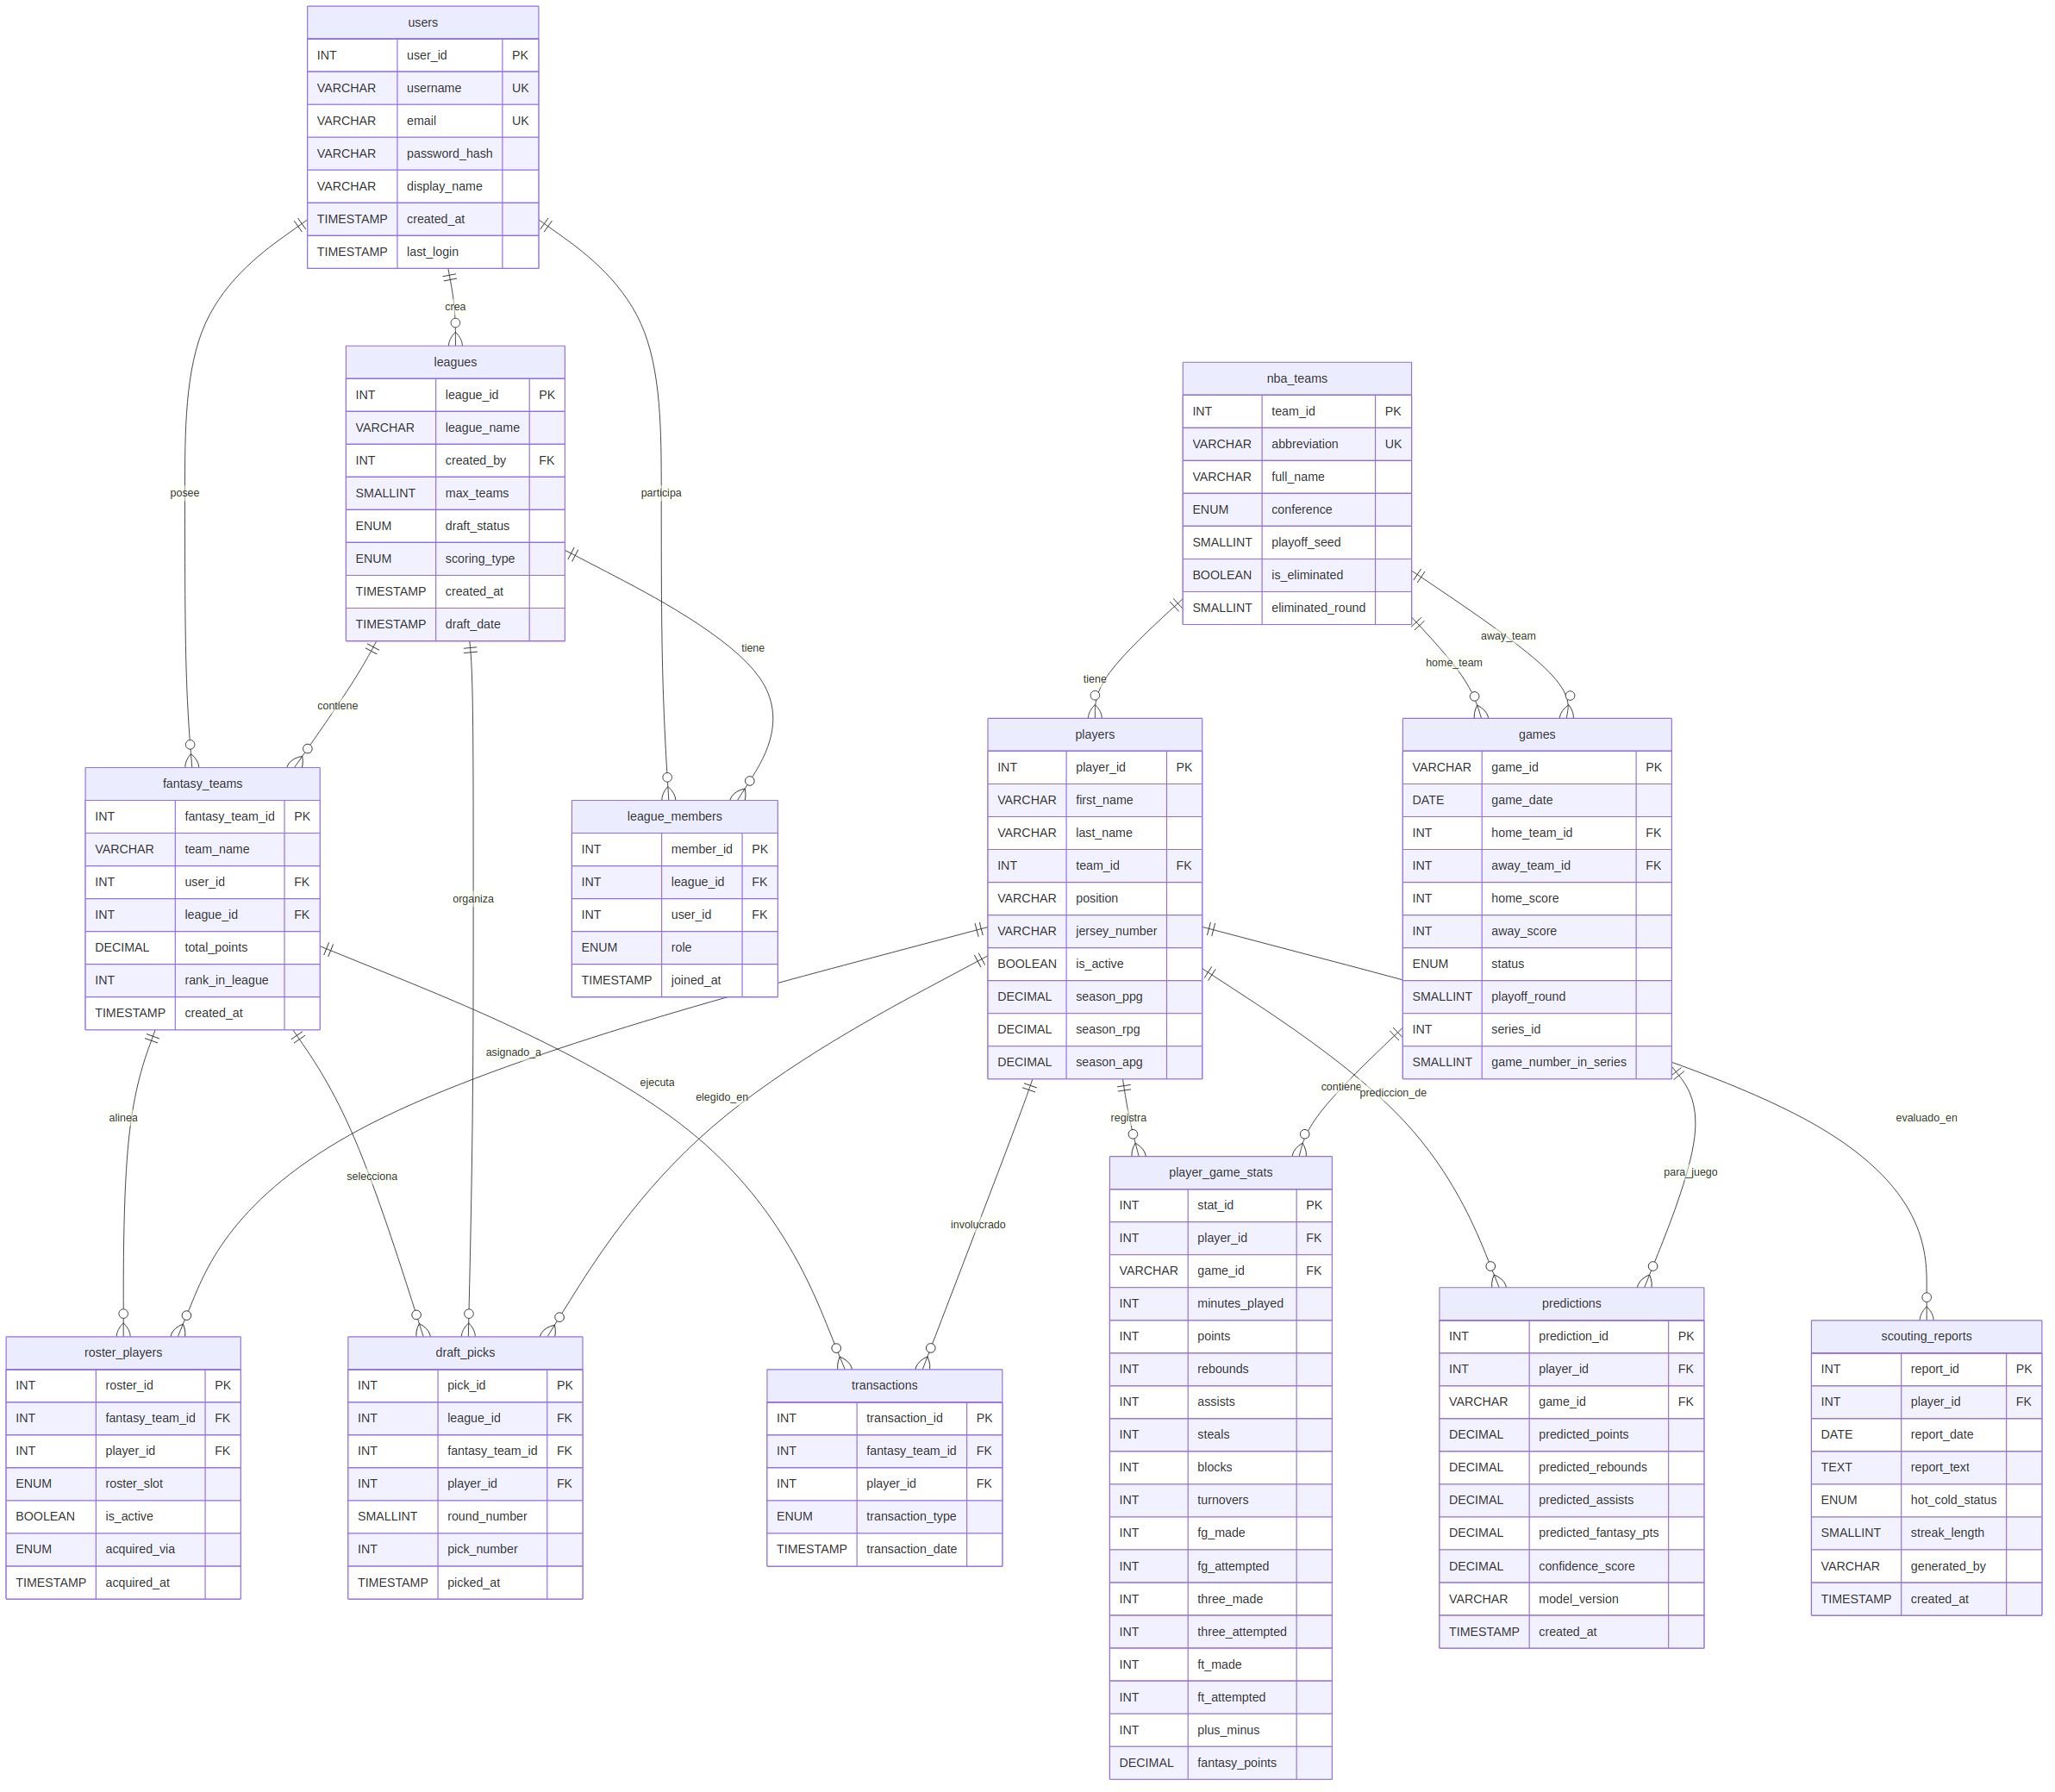
\includegraphics[width=\textwidth]{DER.png}
    \caption{Diagrama Entidad-Relaci\'on --- Playoff Hoops (13 tablas, 20 relaciones FK)}
    \label{fig:der}
\end{figure}

% =============================================================
% 4.2 TABLAS
% =============================================================
\subsection{Descripci\'on de Tablas}

El esquema contiene \textbf{13 tablas}: 10 entidades y 3 junciones muchos-a-muchos.
Se utiliza \texttt{GENERATED ALWAYS AS IDENTITY} para claves primarias autogeneradas,
y IDs oficiales de la NBA para equipos (\texttt{team\_id}) y jugadores (\texttt{player\_id}).

\subsubsection{Tablas de Entidad}

\begin{longtable}{>{\ttfamily\small}p{3.5cm} p{4cm} p{7cm}}
\toprule
\normalfont\textbf{Tabla} & \textbf{PK} & \textbf{Descripci\'on} \\
\midrule
\endhead
users & user\_id (IDENTITY) & Usuarios del sistema. Almacena credenciales (bcrypt hash), nombre de display, timestamps de creaci\'on y \'ultimo login. \\[6pt]
nba\_teams & team\_id (NBA ID) & 30 equipos NBA reales. Incluye conferencia (ENUM East/West), semilla de playoff, estado de eliminaci\'on y ronda en que fueron eliminados. \\[6pt]
players & player\_id (NBA ID) & Jugadores NBA activos. FK a \texttt{nba\_teams}. Almacena posici\'on, n\'umero de jersey, promedios de temporada (PPG, RPG, APG) recalculados diariamente. \\[6pt]
games & game\_id (NBA ID) & Partidos NBA. Dos FKs a \texttt{nba\_teams} (home/away) con CHECK \texttt{home\_team\_id <> away\_team\_id}. Incluye ronda de playoff (1--4), score y estado. \\[6pt]
leagues & league\_id (IDENTITY) & Ligas fantasy creadas por usuarios. FK a \texttt{users} (creador). Configuraci\'on: m\'ax equipos (2--10), tipo de scoring, estado del draft. \\[6pt]
fantasy\_teams & fantasy\_team\_id (IDENTITY) & Equipo fantasy. UNIQUE(user\_id, league\_id) garantiza un equipo por usuario por liga. \texttt{total\_points} mantenido autom\'aticamente por trigger. \\[6pt]
draft\_picks & pick\_id (IDENTITY) & Historial inmutable de selecciones del draft. UNIQUE(league\_id, player\_id) previene doble selecci\'on. UNIQUE(league\_id, pick\_number) previene colisi\'on de turno. \\[6pt]
transactions & transaction\_id (IDENTITY) & Log de movimientos de roster (add/drop/trade). Provee auditor\'ia completa de cambios. \\[6pt]
predictions & prediction\_id (IDENTITY) & Predicciones generadas por el modelo XGBoost. Almacena puntos predichos, rebounds, asistencias, fantasy points, score de confianza y versi\'on del modelo. \\[6pt]
scouting\_reports & report\_id (IDENTITY) & Reportes de texto generados por Claude Haiku. Incluye estado de racha (hot/neutral/cold), longitud de racha y fecha. Cacheados por (player, date). \\
\bottomrule
\end{longtable}

\subsubsection{Tablas de Junci\'on M:M (con atributos --- no diccionarios)}

Cada tabla de junci\'on contiene atributos significativos que justifican su existencia
m\'as all\'a de las dos claves for\'aneas:

\begin{longtable}{>{\ttfamily\small}p{3.5cm} p{3.5cm} p{7cm}}
\toprule
\normalfont\textbf{Junci\'on} & \textbf{Relaciona} & \textbf{Atributos propios} \\
\midrule
\endhead
player\_game\_stats & players $\leftrightarrow$ games &
    \textbf{15 atributos:} minutes\_played, points, rebounds, assists, steals, blocks, turnovers,
    fg\_made, fg\_attempted, three\_made, three\_attempted, ft\_made, ft\_attempted, plus\_minus,
    fantasy\_points (calculado por trigger). \\[6pt]
league\_members & users $\leftrightarrow$ leagues &
    \textbf{role} (commissioner/member), \textbf{joined\_at} (timestamp de uni\'on a la liga). \\[6pt]
roster\_players & fantasy\_teams $\leftrightarrow$ players &
    \textbf{roster\_slot} (G1, G2, F1, F2, C, UTIL, BN1, BN2), \textbf{is\_active} (desactivado si equipo NBA eliminado),
    \textbf{acquired\_via} (draft/free\_agent/trade), \textbf{acquired\_at}. \\
\bottomrule
\end{longtable}

\subsubsection{Cardinalidades}

\begin{longtable}{p{6cm} c p{6cm}}
\toprule
\textbf{Relaci\'on} & \textbf{Card.} & \textbf{Descripci\'on} \\
\midrule
\endhead
nba\_teams $\to$ players & 1:N & Un equipo tiene muchos jugadores \\
nba\_teams $\to$ games (home) & 1:N & Un equipo juega muchos partidos como local \\
nba\_teams $\to$ games (away) & 1:N & Un equipo juega muchos partidos como visitante \\
players $\leftrightarrow$ games & M:N & V\'ia \texttt{player\_game\_stats} (15 attrs) \\
users $\to$ leagues (created\_by) & 1:N & Un usuario crea muchas ligas \\
users $\leftrightarrow$ leagues & M:N & V\'ia \texttt{league\_members} (role, joined\_at) \\
users $\to$ fantasy\_teams & 1:N & Un usuario posee equipos fantasy \\
leagues $\to$ fantasy\_teams & 1:N & Una liga contiene equipos \\
fantasy\_teams $\leftrightarrow$ players & M:N & V\'ia \texttt{roster\_players} (slot, via, active) \\
leagues $\to$ draft\_picks & 1:N & Una liga tiene picks de draft \\
fantasy\_teams $\to$ draft\_picks & 1:N & Un equipo hace picks \\
fantasy\_teams $\to$ transactions & 1:N & Un equipo ejecuta transacciones \\
players $\to$ predictions & 1:N & Un jugador tiene predicciones \\
games $\to$ predictions & 1:N & Un juego tiene predicciones \\
players $\to$ scouting\_reports & 1:N & Un jugador tiene reportes de scouting \\
\bottomrule
\end{longtable}

\subsubsection{Tipos ENUM}

Se definen 9 tipos ENUM para restringir dominios:

\begin{longtable}{>{\ttfamily\small}p{4cm} p{9cm}}
\toprule
\normalfont\textbf{Tipo ENUM} & \textbf{Valores} \\
\midrule
\endhead
conference\_enum & East, West \\
game\_status\_enum & scheduled, live, final \\
draft\_status\_enum & pending, in\_progress, completed \\
scoring\_type\_enum & points, categories \\
member\_role\_enum & commissioner, member \\
roster\_slot\_enum & G1, G2, F1, F2, C, UTIL, BN1, BN2 \\
acquired\_via\_enum & draft, free\_agent, trade \\
txn\_type\_enum & add, drop, trade \\
streak\_status\_enum & hot, neutral, cold \\
\bottomrule
\end{longtable}

% =============================================================
% 4.3 VISTAS
% =============================================================
\subsection{Vistas (6 implementadas, r\'ubrica exige m\'inimo 5)}

\subsubsection{V1: \texttt{v\_league\_leaderboard} --- Tabla de posiciones por liga}

Calcula el ranking en tiempo real de cada equipo fantasy dentro de su liga usando
la funci\'on de ventana \texttt{RANK()}.

\begin{lstlisting}
SELECT ft.team_name, u.username, l.league_name, ft.total_points,
       RANK() OVER (PARTITION BY ft.league_id
                    ORDER BY ft.total_points DESC) AS league_rank,
       COUNT(rp.roster_id) FILTER (WHERE rp.is_active) AS active_roster_size
FROM fantasy_teams ft
JOIN users u ON ft.user_id = u.user_id
JOIN leagues l ON ft.league_id = l.league_id
LEFT JOIN roster_players rp ON ft.fantasy_team_id = rp.fantasy_team_id
GROUP BY ft.fantasy_team_id, ...;
\end{lstlisting}

\textbf{Justificaci\'on:} Reporte principal de cualquier liga. \texttt{RANK()} maneja empates correctamente
(dos equipos con el mismo puntaje obtienen el mismo rango).

\subsubsection{V2: \texttt{v\_player\_performance} --- Rendimiento agregado por jugador}

Calcula promedios de temporada (puntos, rebotes, asistencias, fantasy points) agrupados por jugador.

\begin{lstlisting}
SELECT p.first_name || ' ' || p.last_name AS player_name,
       COUNT(pgs.stat_id) AS games_played,
       ROUND(AVG(pgs.points)::numeric, 1) AS avg_pts,
       ROUND(AVG(pgs.fantasy_points)::numeric, 1) AS avg_fantasy_pts,
       ROUND(SUM(pgs.fantasy_points)::numeric, 1) AS total_fantasy_pts
FROM players p
JOIN nba_teams t ON p.team_id = t.team_id
LEFT JOIN player_game_stats pgs ON p.player_id = pgs.player_id
GROUP BY p.player_id, ...;
\end{lstlisting}

\textbf{Justificaci\'on:} Alimenta la b\'usqueda de jugadores en el front-end y provee datos
para el modelo de predicci\'on.

\subsubsection{V3: \texttt{v\_hot\_cold\_players} --- Detecci\'on de rachas}

Usa un \textbf{CTE} con \texttt{ROW\_NUMBER()} para aislar los \'ultimos 5 partidos de cada jugador
y compararlos contra su media de temporada. Clasifica como \texttt{hot} ($>$+20\%), \texttt{cold} ($<$-20\%)
o \texttt{neutral}.

\begin{lstlisting}
WITH last5 AS (
    SELECT pgs.player_id, pgs.points,
           ROW_NUMBER() OVER (PARTITION BY pgs.player_id
                              ORDER BY g.game_date DESC) AS rn
    FROM player_game_stats pgs JOIN games g ON pgs.game_id = g.game_id
)
SELECT p.player_name, p.season_ppg,
       AVG(l.points) AS last5_ppg,
       CASE WHEN AVG(l.points) > season_ppg * 1.20 THEN 'hot'
            WHEN AVG(l.points) < season_ppg * 0.80 THEN 'cold'
            ELSE 'neutral' END AS streak_status
FROM players p JOIN last5 l ON p.player_id = l.player_id AND l.rn <= 5
GROUP BY ...;
\end{lstlisting}

\textbf{Justificaci\'on:} Diferenciador clave del proyecto. Ninguna plataforma existente ofrece
esta m\'etrica integrada en el sistema de fantasy. Utiliza CTE y funciones de ventana.

\subsubsection{V4: \texttt{v\_roster\_detail} --- Composici\'on del roster}

JOIN de 5 tablas (\texttt{fantasy\_teams}, \texttt{users}, \texttt{roster\_players}, \texttt{players}, \texttt{nba\_teams})
para mostrar la composici\'on completa de cada equipo fantasy con el slot asignado, estado activo/inactivo
y promedios del jugador.

\textbf{Justificaci\'on:} P\'agina principal de gesti\'on de roster en el front-end.

\subsubsection{V5: \texttt{v\_daily\_scoring} --- Scoring diario con multiplicador}

Presenta el desglose de puntos de cada jugador por partido con el multiplicador de ronda
aplicado: R1 $\times$1.0, Semis $\times$1.25, Conference Finals $\times$1.5, NBA Finals $\times$2.0.

\textbf{Justificaci\'on:} Implementa el diferenciador central del sistema (puntos progresivos por ronda).

\subsubsection{V6: \texttt{v\_prediction\_accuracy} --- Precisi\'on del modelo ML}

Calcula el \textbf{MAE} (Mean Absolute Error) entre predicciones del modelo XGBoost y resultados reales,
agrupado por jugador y versi\'on del modelo.

\textbf{Justificaci\'on:} Permite evaluar y comparar iteraciones del modelo de predicci\'on.

% =============================================================
% 4.4 STORED PROCEDURES
% =============================================================
\subsection{Stored Procedures (9 implementados)}

Todos los procedures utilizan \textbf{esquema transaccional con COMMIT expl\'icito}.
Si cualquier statement falla antes del COMMIT, PostgreSQL ejecuta ROLLBACK autom\'atico.

\textbf{Nota t\'ecnica:} Los procedures que usan COMMIT no pueden tener bloques \texttt{EXCEPTION}
porque \'estos abren subtransacciones incompatibles con el control de transacci\'on expl\'icito.

\subsubsection{Funci\'on auxiliar: \texttt{fn\_compute\_fantasy\_pts}}

Funci\'on \texttt{IMMUTABLE} que calcula fantasy points con la f\'ormula:

$$FP = (PTS \times 1.0) + (REB \times 1.2) + (AST \times 1.5) + (STL \times 2.0) + (BLK \times 2.0) + (3PM \times 0.5) - (TOV \times 1.0)$$

Con bonificaciones:
\begin{itemize}[nosep]
    \item \textbf{Double-Double} ($\geq$2 categor\'ias $\geq$10): +1.5 puntos
    \item \textbf{Triple-Double} ($\geq$3 categor\'ias $\geq$10): +3.0 puntos
\end{itemize}

Y multiplicador por ronda: R1 $\times$1.00, R2 $\times$1.25, R3 $\times$1.50, R4 $\times$2.00.

\subsubsection{Procedures INSERT (3)}

\begin{longtable}{>{\ttfamily\small}p{4.5cm} p{9cm}}
\toprule
\normalfont\textbf{Procedure} & \textbf{Descripci\'on} \\
\midrule
sp\_register\_user & Registra un usuario nuevo. Retorna \texttt{user\_id} via \texttt{INOUT}. COMMIT al final. \\[4pt]
sp\_create\_league & Crea liga + agrega al creador como \texttt{commissioner} en \texttt{league\_members}. \textbf{At\'omico:} ambas operaciones o ninguna. \\[4pt]
sp\_make\_draft\_pick & Pick de draft con \textbf{bloqueo pesimista} (\texttt{SELECT FOR UPDATE}) para evitar doble pick concurrente. Inserta en \texttt{draft\_picks} y \texttt{roster\_players} at\'omicamente. \\
\bottomrule
\end{longtable}

\subsubsection{Procedures UPDATE (2)}

\begin{longtable}{>{\ttfamily\small}p{5.5cm} p{8cm}}
\toprule
\normalfont\textbf{Procedure} & \textbf{Descripci\'on} \\
\midrule
sp\_update\_player\_game\_stats & Actualiza stats de un jugador y recalcula \texttt{fantasy\_points} usando \texttt{fn\_compute\_fantasy\_pts}. \\[4pt]
sp\_calculate\_fantasy\_points & Recalcula \texttt{fantasy\_points} por \texttt{stat\_id}. Lee stats actuales, aplica f\'ormula, actualiza. \\
\bottomrule
\end{longtable}

\subsubsection{Procedures DELETE (3)}

\begin{longtable}{>{\ttfamily\small}p{5cm} p{8.5cm}}
\toprule
\normalfont\textbf{Procedure} & \textbf{Descripci\'on} \\
\midrule
sp\_delete\_fantasy\_team & Elimina equipo fantasy con cascada controlada. Loggea cada drop en \texttt{transactions} antes de eliminar roster, picks y equipo. \\[4pt]
sp\_drop\_roster\_player & Drop individual. Valida existencia, registra en \texttt{transactions}, elimina de \texttt{roster\_players}. \\[4pt]
sp\_leave\_league & Abandono de liga. Cascade: drops loggeados $\to$ roster limpio $\to$ picks eliminados $\to$ equipo eliminado $\to$ members\'ia removida. \\
\bottomrule
\end{longtable}

\subsubsection{Procedure complejo: \texttt{sp\_free\_agent\_swap}}

Swap at\'omico de free agent (drop + add en una sola transacci\'on):

\begin{lstlisting}
CREATE OR REPLACE PROCEDURE sp_free_agent_swap(
    p_fantasy_team_id INT, p_drop_player_id INT, p_add_player_id INT
) LANGUAGE plpgsql AS $$
DECLARE v_slot roster_slot_enum;
BEGIN
    -- Bloqueo pesimista: lock la fila del jugador a soltar
    SELECT roster_slot INTO v_slot FROM roster_players
     WHERE fantasy_team_id = p_fantasy_team_id
       AND player_id = p_drop_player_id FOR UPDATE;
    IF v_slot IS NULL THEN
        RAISE EXCEPTION 'Player % not on roster', p_drop_player_id;
    END IF;
    -- Drop
    DELETE FROM roster_players WHERE fantasy_team_id = p_fantasy_team_id
       AND player_id = p_drop_player_id;
    -- Add (hereda el mismo slot)
    INSERT INTO roster_players (fantasy_team_id, player_id, roster_slot, acquired_via)
    VALUES (p_fantasy_team_id, p_add_player_id, v_slot, 'free_agent');
    -- Log ambos movimientos
    INSERT INTO transactions (fantasy_team_id, player_id, transaction_type) VALUES
        (p_fantasy_team_id, p_drop_player_id, 'drop'),
        (p_fantasy_team_id, p_add_player_id,  'add');
    COMMIT;
END $$;
\end{lstlisting}

\textbf{Justificaci\'on:} Demuestra transacci\'on compleja con bloqueo pesimista, m\'ultiples
tablas afectadas (3: \texttt{roster\_players}, \texttt{transactions} $\times$2), y atomicidad cr\'itica
(no puede existir un momento donde el jugador fue soltado pero el reemplazo no fue agregado).

% =============================================================
% 4.5 TRIGGERS
% =============================================================
\subsection{Triggers (5 implementados)}

\subsubsection{T1: \texttt{trg\_calc\_fp\_on\_insert} --- C\'alculo autom\'atico de fantasy points}

\textbf{Tipo:} \texttt{BEFORE INSERT} en \texttt{player\_game\_stats}.

Cada vez que se inserta una nueva fila de estad\'isticas, el trigger invoca
\texttt{fn\_compute\_fantasy\_pts()} y asigna el resultado a \texttt{NEW.fantasy\_points}
antes de que la fila se escriba en disco.

\textbf{Justificaci\'on:} Garantiza que \texttt{fantasy\_points} siempre est\'e sincronizado con las
stats sin depender del c\'odigo de aplicaci\'on.

\subsubsection{T2: \texttt{trg\_update\_team\_points} --- Actualizaci\'on de puntaje total}

\textbf{Tipo:} \texttt{AFTER INSERT OR UPDATE OF fantasy\_points} en \texttt{player\_game\_stats}.

Recalcula \texttt{fantasy\_teams.total\_points} sumando los \texttt{fantasy\_points} de todos los
jugadores activos en el roster. Solo afecta equipos que tienen al jugador modificado.

\textbf{Justificaci\'on:} Mantiene el leaderboard actualizado en tiempo real sin queries costosos.

\subsubsection{T3: \texttt{trg\_eliminate\_team} --- Cascada de eliminaci\'on}

\textbf{Tipo:} \texttt{AFTER UPDATE OF is\_eliminated} en \texttt{nba\_teams}.

Cuando un equipo NBA es eliminado del playoff (\texttt{is\_eliminated} pasa de FALSE a TRUE),
desactiva autom\'aticamente (\texttt{is\_active = FALSE}) a todos sus jugadores en todos los rosters fantasy.

\textbf{Justificaci\'on:} Regla de negocio cr\'itica --- jugadores de equipos eliminados no deben seguir generando puntos.

\subsubsection{T4: \texttt{trg\_check\_roster\_size} --- Validaci\'on de tama\~no de roster}

\textbf{Tipo:} \texttt{BEFORE INSERT} en \texttt{roster\_players}.

Impide que un equipo fantasy tenga m\'as de 8 jugadores en su roster.
Lanza \texttt{RAISE EXCEPTION} si se intenta exceder el l\'imite.

\textbf{Justificaci\'on:} Constraint de negocio que no puede expresarse con CHECK est\'andar
(requiere contar filas en la misma tabla).

\subsubsection{T5: \texttt{trg\_validate\_last\_login} --- Validaci\'on de login}

\textbf{Tipo:} \texttt{BEFORE UPDATE OF last\_login} en \texttt{users}.

Impide que \texttt{last\_login} se establezca a una fecha futura.

\textbf{Justificaci\'on:} Previene inconsistencias temporales en auditor\'ia de acceso.

% =============================================================
% 4.6 DATOS REALES
% =============================================================
\subsection{Datos Reales Cargados}

La base de datos contiene estad\'isticas reales de la NBA, actualizadas diariamente
mediante un pipeline automatizado:

\begin{table}[h!]
\centering
\begin{tabular}{lrrl}
\toprule
\textbf{Temporada} & \textbf{Games} & \textbf{Stats} & \textbf{Fuente} \\
\midrule
2023-24 & 1,230 & 21,102 & nba\_api (PlayerGameLog) \\
2024-25 & 1,314 & 44,848 & Kaggle (eoinamoore) \\
2025-26 & 1,232 & 22,597 & Kaggle (eoinamoore) \\
\midrule
\textbf{Total} & \textbf{3,776} & \textbf{88,547} & \\
\bottomrule
\end{tabular}
\caption{Resumen de datos cargados por temporada}
\end{table}

\begin{itemize}[nosep]
    \item \textbf{30} equipos NBA reales.
    \item \textbf{791} jugadores con estad\'isticas de box score.
    \item \textbf{84} partidos de playoffs 2024-25 con rondas correctamente asignadas (R1--R4).
    \item Actualizaci\'on diaria autom\'atica v\'ia \texttt{cron} + Kaggle CLI.
\end{itemize}

% =============================================================
% 4.7 NORMALIZACIÓN
% =============================================================
\subsection{Normalizaci\'on --- FNBC}

El esquema cumple con la \textbf{Forma Normal de Boyce-Codd (FNBC)}:

\begin{itemize}
    \item \textbf{1FN:} Todos los atributos son at\'omicos. No hay grupos repetidos ni arrays.
    \item \textbf{2FN:} No hay dependencias parciales. Cada atributo no-clave depende de la clave
          primaria completa (relevante en junciones como \texttt{player\_game\_stats} donde la PK
          es \texttt{stat\_id} y el UNIQUE constraint es (\texttt{player\_id, game\_id})).
    \item \textbf{3FN:} No hay dependencias transitivas. Por ejemplo, \texttt{conference} depende
          de \texttt{team\_id} (no transitivamente de \texttt{player\_id}).
    \item \textbf{FNBC:} Todo determinante es clave candidata. Los atributos derivados
          (\texttt{fantasy\_points}, \texttt{total\_points}) son mantenidos por triggers,
          no por dependencias funcionales.
\end{itemize}

% =============================================================
% 5. CONCLUSIONES
% =============================================================
\section{Conclusiones}

\begin{enumerate}
    \item El esquema en FNBC con 13 tablas, 20 relaciones FK, 3 junciones M:M con atributos
          y 9 tipos ENUM proporciona una base s\'olida para el sistema de fantasy basketball.

    \item Los 9 stored procedures transaccionales con COMMIT expl\'icito demuestran el manejo
          completo de operaciones INSERT, UPDATE y DELETE con atomicidad garantizada,
          incluyendo bloqueo pesimista (\texttt{SELECT FOR UPDATE}) para concurrencia.

    \item Los 5 triggers mantienen la consistencia de datos derivados (fantasy points, puntaje
          total, eliminaci\'on en cascada) sin depender de la l\'ogica de aplicaci\'on.

    \item Las 6 vistas con funciones de ventana (\texttt{RANK}, \texttt{ROW\_NUMBER}), CTEs
          y agregaciones proveen los reportes anal\'iticos requeridos por el front-end.

    \item La carga de 88,547 estad\'isticas reales de 3 temporadas NBA valida que el esquema
          soporta volumen de datos real y permite entrenar modelos predictivos con datos actuales.

    \item El pipeline de actualizaci\'on diaria (cron + Kaggle) asegura que el sistema refleja
          los resultados m\'as recientes de la NBA, diferenci\'andolo de soluciones est\'aticas.
\end{enumerate}

% =============================================================
% 6. ÉTICA GEN AI
% =============================================================
\section{Declaraci\'on de Uso de IA Generativa}

De acuerdo con la pol\'itica de \'etica del curso, se declara que se utiliz\'o \textbf{Claude Code}
(Anthropic, modelo Claude Opus) como herramienta de asistencia para:

\begin{itemize}[nosep]
    \item Generaci\'on de boilerplate SQL (CREATE TABLE, tipos ENUM).
    \item Depuraci\'on de errores de PL/pgSQL (subtransacciones, conflictos de firma de procedures).
    \item Escritura de scripts de seed de datos (Python con nba\_api y Kaggle).
    \item Generaci\'on de este informe en \LaTeX.
\end{itemize}

Todas las decisiones de dise\~no (elecci\'on de FNBC, cardinalidades, f\'ormula de fantasy points,
estructura de triggers, selecci\'on de PostgreSQL sobre MySQL) fueron tomadas por el estudiante
y pueden ser defendidas en la presentaci\'on oral.

\end{document}
